\documentclass[preview]{standalone}

\usepackage{graphicx}
\usepackage[showframe]{geometry}
\geometry{
paperwidth=11cm,
paperheight=5cm,
margin=0cm
}

\usepackage[dvipsnames]{xcolor}
\usepackage{tikz}
\newcommand{\probplotvalue}[1]{%
    \definecolor{probvalcolor}{RGB}{#1}%
    \definecolor{outlinecolor}{RGB}{127, 127, 127}%
    \begin{tikzpicture}[baseline={([yshift=-.5ex]current bounding box.center)}]%
        \pgfmathsetmacro{\size}{0.25};%
        \draw[outlinecolor, fill=probvalcolor] (-\size,-\size) -- (-\size, +\size) -- (+\size, +\size) -- (+\size, -\size) -- cycle;%
    \end{tikzpicture}%
}%
\begin{document}
    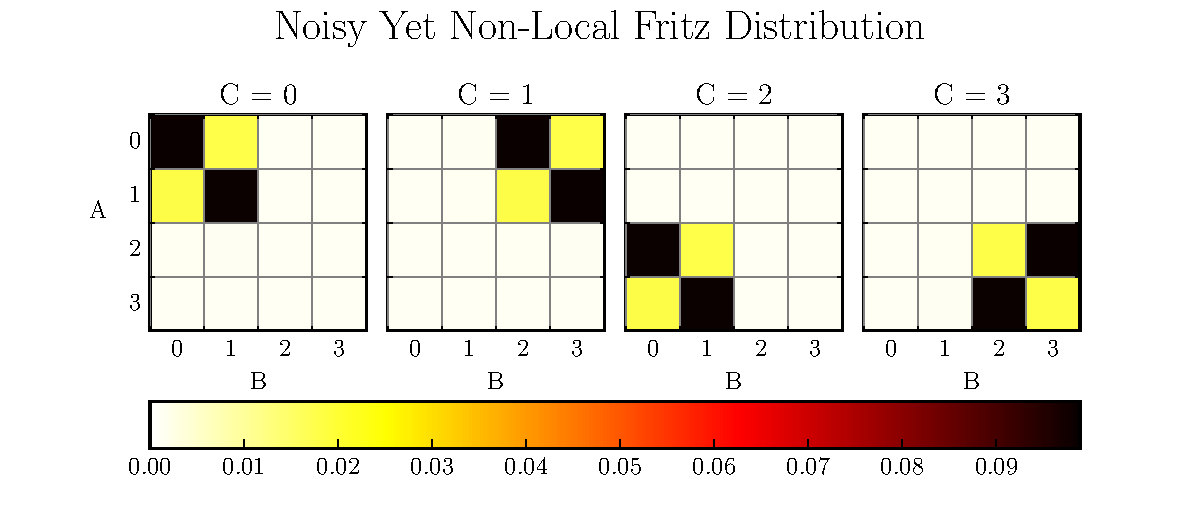
\includegraphics[scale=0.6,trim={1cm 2.2cm 1cm 0.4in},clip]{noisy_yet_non_local_fritz_uncropped.pdf}
    \[ \probplotvalue{253, 253, 84} = 0.018 \qquad \probplotvalue{11, 1, 0} = 0.099 \qquad \probplotvalue{255, 255, 243} = 0.0013 \]
    \vspace{0cm} %whitespace hack
\end{document}